\section{Introduction}
\label{sec:intro}

BGP~\cite{bgp}, the protocol used for inter-domain internet routing,
can be disrupted by a wide range of attacks and accidental
misconfigurations~\cite{s-bgp1,s-bgp3,threat}. Spammers hijack address spaces to increase their ability to send vast quantities of unsolicited email. Changes in BGP configuration can have unintended consequences, such as accidentally marking one's system the best route to every other system; this `black hole' will attract and drop a large portion of the internet's traffic. As the internet has
become vitally important to worldwide communication and commerce,
disruptions such as these have become unacceptable. In order to secure BGP, most
researchers recommend that infrastructure, typically an address space
PKI, be instituted for determining whether routes were originated by
authorized parties~\cite{s-bgp1,s-bgp2,sobgp,psbgp,spv}. This PKI will
allow the owner of an address space, and only that owner, to advertise
information about it. In order to do this, the party managing the
address space signs data stating that some party may manage that
address space. That managing party may then delegate responsibility to
sub-parties and so on. We illustrate part of this proposed hierarchy
in Figure~\ref{fig:hierarchy}. As such, the root of this address PKI
should be the organization which is responsible for the disposition of
the addresses.

\begin{figure}
\begin{center}
\fbox{
\begin{minipage}{5in}
\centerline{
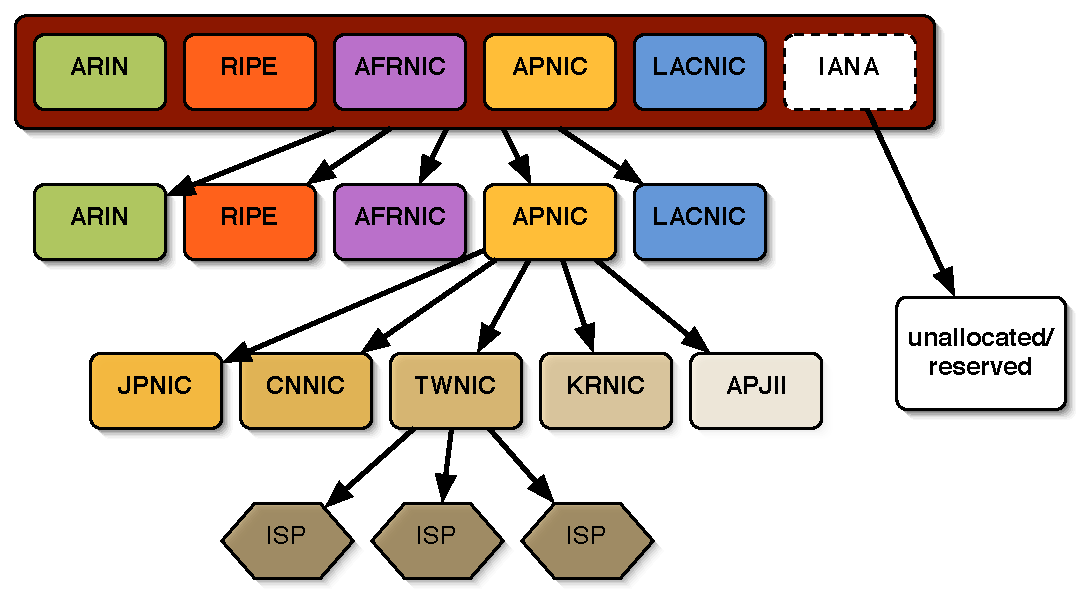
\includegraphics[width=5in]{figures/pki-hierarchy} 
}
\end{minipage}

}% FBOX
\end{center}
\caption{\small The address PKI root should be managed by the five RIRs in collaboration with IANA. The root of the hierarchy signs certificates allowing each RIR to securely manage its allocated address space. Each RIR, in turn, signs certificates for the address allocations of  ISPs and/or country registries, who may delegate sections of the address space in turn.}
\label{fig:hierarchy}
\end{figure}

% TODO - DNSsec

The nominal root of the address distribution hierarchy could be considered either the Internet Assigned Numbers Authority (IANA) or the Number Resource Organization (NRO). However, neither is engaged in daily operational concerns. As compromising the root of the address PKI allows an attacker to negate the security gained from the PKI, the root signing key must be highly protected. While IANA or NRO might not be set up well to run the PKI root, the five Regional Internet Registries (RIR) have a suitable operational and security setup. None of them, however, should control the worldwide address registry; instead, they can share responsibility for acting as the PKI root.

DNS has been subject to spoofing attacks and misconfiguration in much the same manner as BGP. To defend against these attacks, DNSsec~\cite{dnssec} allows parties responsible for DNS names to certify information about those names. Unfortunately, there is currently no DNSsec trust root, only disconnected trust anchors. Political and technical challenges have prevented the creation of such a root. Our technical solution to the problems of an address space root seem to apply equally well to a DNSsec root, despite the greater logistical complexity implied by the larger number of stakeholders. Instead of the RIRs sharing responsibility for the root, the twelve root server operators can jointly operate the DNSsec root, signing certificates for the over 160 top level domain administrators. For simplicity, we discuss our solution only in terms of the address space PKI in the remainder of this paper, though it is also applicable to the DNSsec system.

There are three basic ways of distributing responsibility for the address PKI root. Each RIR could run its own root, with which it signs data relating to its area of responsibility. This scheme has a severe disadvantage: distributing five independent root keys will greatly increase the operational complexity of the PKI structure. Instead of having five independent roots, the RIRs could each hold a copy of the PKI root signing key. Unfortunately, this scheme would be more vulnerable to security breaches; leaking any of the five keys is sufficient to break the entire scheme. In addition, administrative snafus in any RIR could cause addresses to be doubly-allocated or accidentally removed.

We recommend instead a scheme that distributes the root key among the five RIRs, several of whom jointly sign data. Distributing the root key has two important benefits: (1) if multiple distributed keys are required to sign data, the PKI root can achieve greater security; (2) if not all players must participate in signing data, the PKI root can achieve greater availability.
We recommend that a majority (three) of the five RIRs be required to sign data; any two RIRs may be unavailable or uncooperative without affecting operations in any way. For clarity, we sketch the key generation and signing procedures of a distributed address-space PKI root in Figure~\ref{fig:sign-combine}. As legacy address allotments do not fall into any RIRs domain, holders of such allotments can be encouraged to move their addresses into the RIR system by not including them in the address PKI and thus excluding them from the protection it provides. Distribution of the DNS root infrastructure has lead in practice to increased security and robustness for that system; we expect the same to be true for address spaces and AS numbers.

\begin{figure}
\begin{center}
\fbox{
\begin{minipage}{5in}
\centerline{
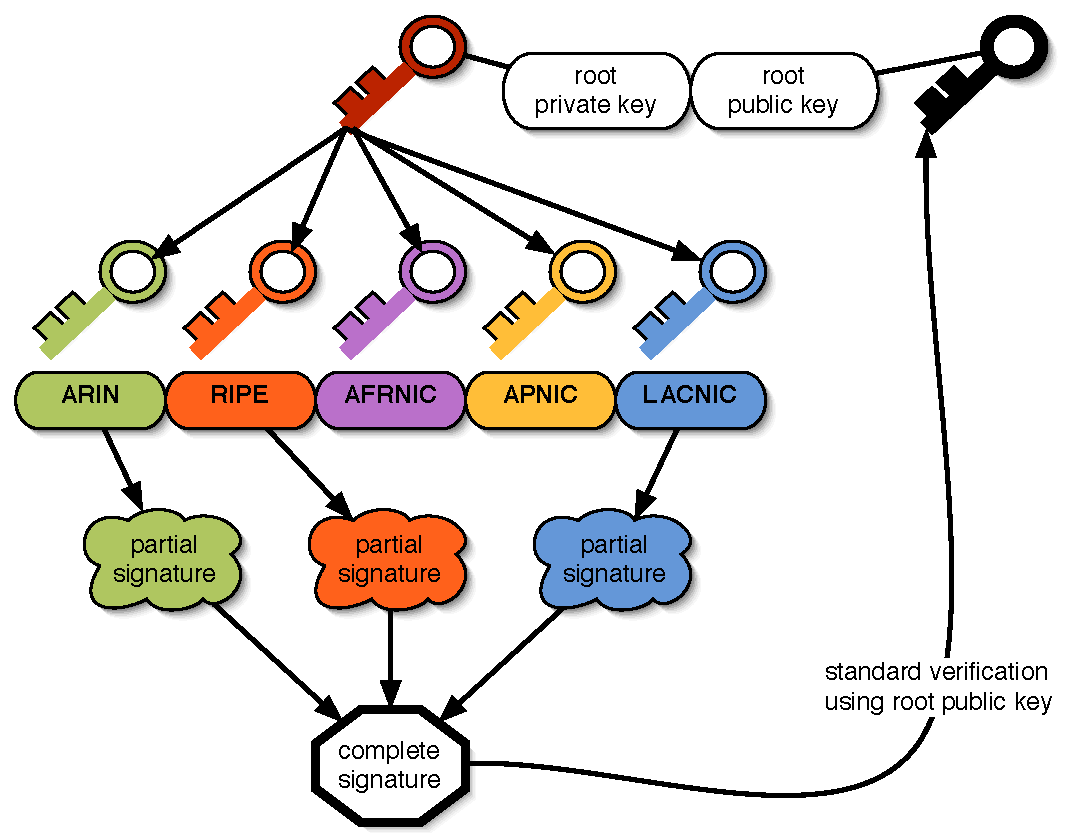
\includegraphics[width=5in]{figures/sign-combine} 
}
\end{minipage}

}% FBOX
\end{center}
\caption{\small The distributed root of a PKI functions as follows: (1) a trusted dealer chooses a root public and private (signing) key; (2) the dealer creates shares of the signing key for each player/RIR; (3) to create a signature, at least \nums\ players create partial signatures from their key shares and combine them into a complete signature; (4) the complete signature can be verified with the root public key, just as if it were created directly from the root private key.}
\label{fig:sign-combine}
\end{figure}

In order to make distribution of the root signing key a practical option, we must design a scheme with the following properties:
\begin{itemize}
\item {\it Transparent.} Verifiers should not need to know what the administrative set-up of the PKI root is. Verification should be as standard as possible.
\item {\it Key refresh.} The members of the root collective should be able to refresh their keys, yielding a new set of private keys corresponding to the same public key. If only two keys have been compromised, key refresh will restore secrecy to the private key shares.
\item {\it Efficient.} The scheme must be efficient in computation and communication, especially in interactive communication. Each member of the root collective should perform its computation in isolation, then send the results ({\it signatures shares}, parts of a signature) to a single player. The single player then performs computation to combine these signature shares into a complete signature, valid under the root public key, without further communication.
\end{itemize}

In this paper, we outline procedural and technical details for a distributed root with these properties based on Shoup's threshold RSA signature scheme~\cite{shoup-sig}.